\section{Demonstration of the UQ package workflow}

This section is a concrete example of how one can use the uncertainty quantification package to improve the quality of the models trained iteratively. Consider a base model for regression trained by the user for which he/she cares about reliable UQ. In this case, it is represented by a CatBoost regression GBT and reaches an R2 of 0.74:

\begin{lstlisting}[language=Python, caption=Base user model.]
def get_base_model():
    return CatBoostRegressor(...)
model = get_base_model()
model.fit(X_train, y_train)
\end{lstlisting}

The first step of the workflow is to use one of the uncertainty wrappers. It is assumed that the user is interested in both data and model uncertainty via a size-5 seed ensemble.

\begin{lstlisting}[language=Python, caption=Step 1: train UQ model.]
from uqlearn.data_uq import DataUQWrapper
from uqlearn.model_uq import ModelUQWrapper

uq_model = ModelUQWrapper(
    DataUQWrapper(model), ensemble='seed', n_estimators=5
)
uq_model.fit(X_train, y_train)
preds, std = uq_model.predict(X_test, return_std=True)
\end{lstlisting}

The updated UQ model can also predict standard deviations. The results are displayed, e.g. via confidence intervals, for the first 5 test data points in figure \ref{fig:demo-viz}. Model uncertainty, which can be viewed as the spread of the x-axis in the top-left plot,  seems to play a notable role in this example, especially for data point 2. In fact, the mean prediction is far from the true value, as highlighted in the bottom-right plot. Overall, the reliability diagram of the model and the ordered prediction intervals can be found in figure \ref{fig:demo-calibration}. The case of data point 2 is not isolated, and most of the predicted confidence intervals are too narrow, which results in a very over-confident and uncalibrated model (miscalibration area of 0.37).

\begin{figure}[!ht]
    \centering
    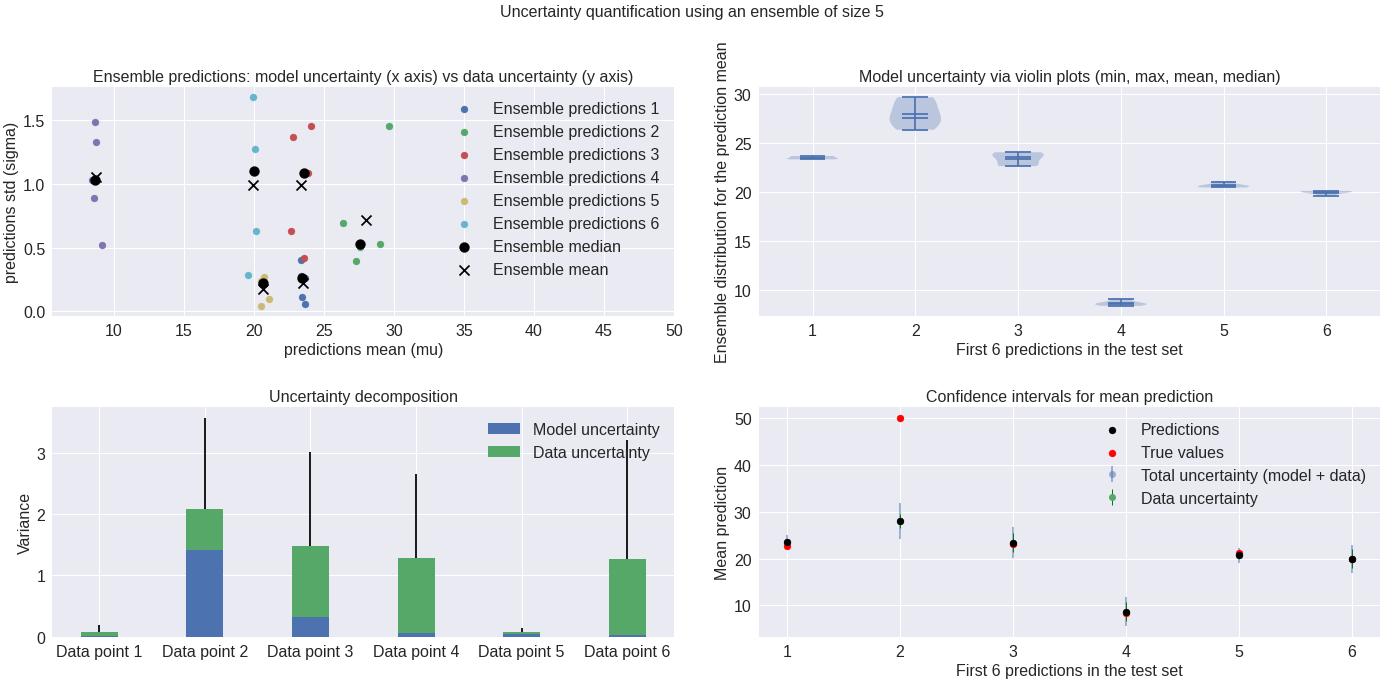
\includegraphics[width=\linewidth]{figures/eval/demo/demo_eval.png}
    \caption{Demo. Evaluation of the first 5 test data points. The top-left plot contains the raw predictions for each member of the ensemble. The bottom-left one highlights how total uncertainty is distributed across its data and model components. Different variations of confidence internals are shared in the two right figures.}
    \label{fig:demo-viz}
\end{figure}

\begin{figure}[!ht]
    \centering
    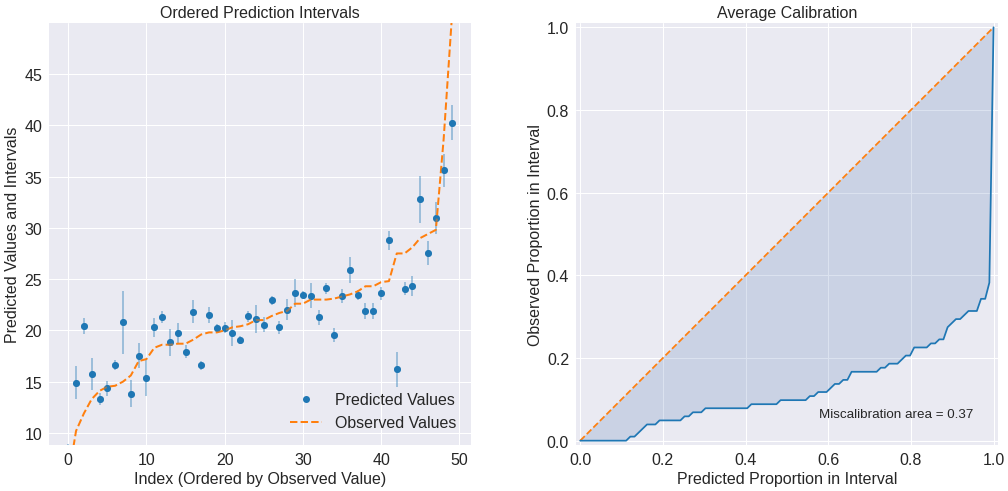
\includegraphics[scale=0.40]{figures/eval/demo/4_evaluation.png}
    \caption{Demo. Reliability plots for the UQ model.}
    \label{fig:demo-calibration}
\end{figure}

The package also offers calibration tools to address this issue. It is the second step of this workflow. The \textit{calibrated\_uq\_model} is better calibrated (cf. figure \ref{fig:demo-recalibration}) and can be trusted regarding uncertainty quantification. The evaluation metrics described in section \ref{metrics:regression} are reported in table \ref{tab:demo:metrics} for both models. 

\begin{lstlisting}[language=Python, caption=Step 2: calibration of UQ model.]
from uqlearn.calibration import CalibratedRegressorCV

calibrated_uq_model = CalibratedRegressorCV(uq_model, cv=4)
calibrated_uq_model.fit(X_train, y_train)
preds, std = calibrated_uq_model.predict(X_test, return_std=True)
\end{lstlisting}


\begin{figure}[h!]
    \centering
    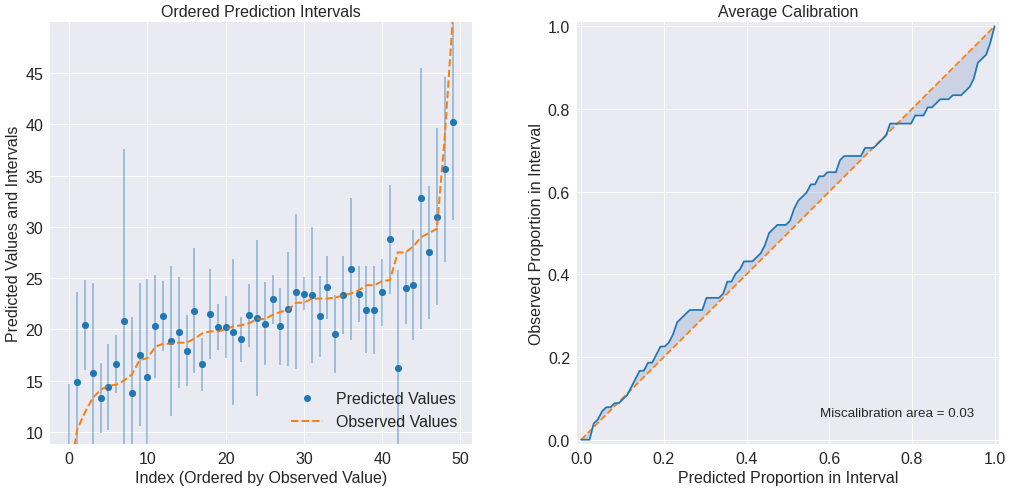
\includegraphics[scale=0.40]{figures/eval/demo/6_calibration_evaluation.png}
    \caption{Demo. Reliability plots for the calibrated UQ model.}
    \label{fig:demo-recalibration}
\end{figure}



\begin{table}[h!]
    \centering
    \begin{tabular}{lrr}
    \toprule
    Metric & Base value & Value after calibration \\
    \midrule
       R2 & 0.74 & 0.74\\
       Coverage score &	0.25 & 0.93 \\
 %      Coverage absolute error & 0.70 & 0.02\\
 %      Width score	& 1.92 & 13.64\\
       NLL &	42.71  & 2.15\\
       Miscalibration area & 0.38 & 0.06 \\
    \bottomrule
    \end{tabular}
    \caption{Demo. Regression UQ evaluation metrics for uncalibrated and calibrated models.}
    \label{tab:demo:metrics}
\end{table}

\section{UQ validity checks}

In this experiment, different UQ models are compared on a regression and a classification dataset: seed, bagging and hyper-parameter ensembles of different sizes, i.e. 10, 20, 30 and 50 members. The models are not re-calibrated using an extra calibration dataset. 



% show plots and example outputs
\subsection{Regression}

Gaussian Process, Random Forest, Gradient-Boosted Trees, Ridge regression, and Bayesian Ridge Regression models are trained on the Boston Housing dataset and evaluated using the following metrics: R2, Miscalibration area ($ECE$), coverage absolute error and Negative Log-Likelihood (NLL). All metrics are independently computed for total, data, and model uncertainties. Besides, data uncertainty is further estimated via an intrinsic and an extrinsic UQ model. The extrinsic model is a quantile regression model trained using cross-validation. %to produce calibration sets. 

\begin{figure}[!ht]
    \centering
    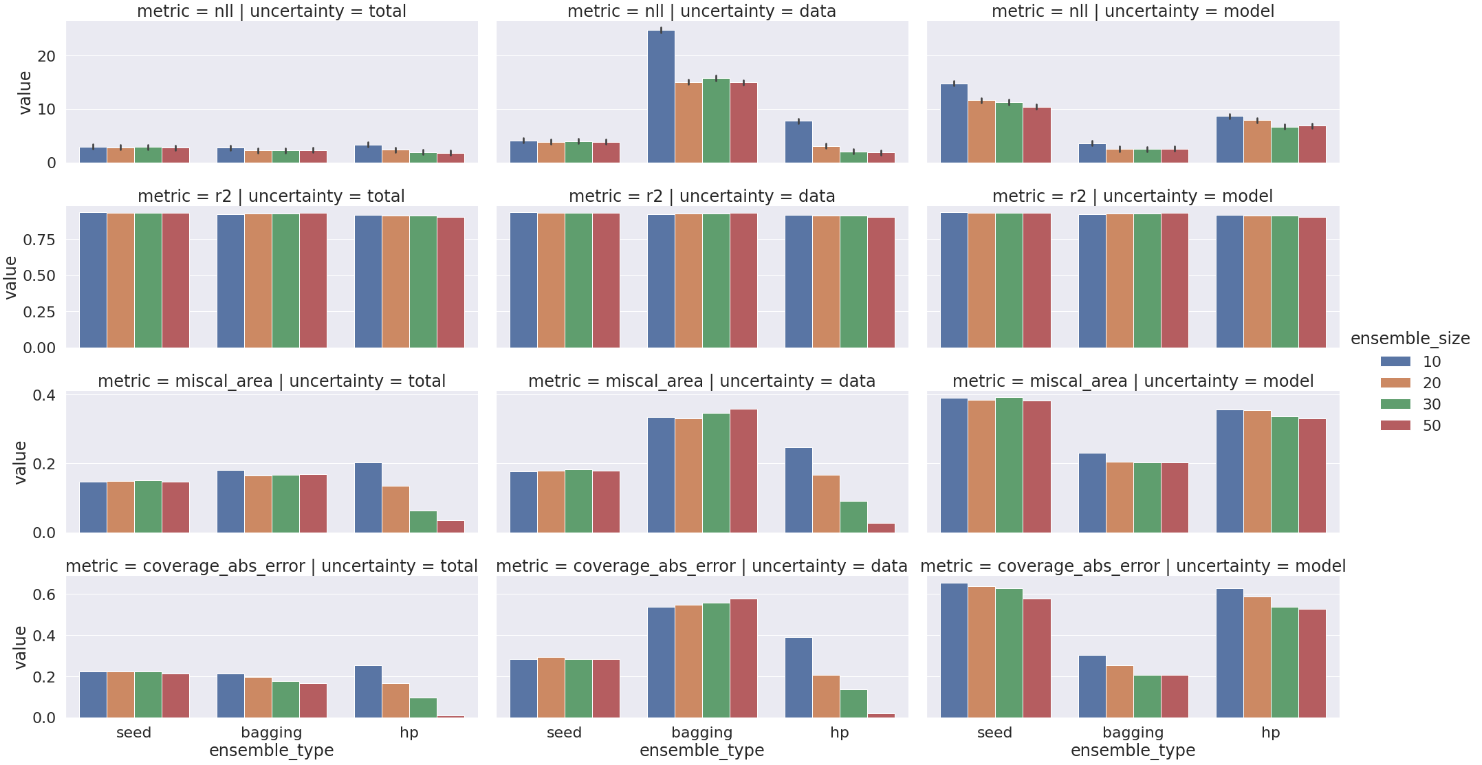
\includegraphics[width=\linewidth]{figures/eval/uqlearn/regression-results.png}
    \caption{Results of regression experiment for CatBoost model.}
    \label{fig:regression-catboost-results}
\end{figure}
Given the large amount of data collected and the size constraints of this thesis, the detailed analysis in figures \ref{fig:regression-catboost-results} and \ref{fig:regression-catboost-heatmap} is only performed for a single base model type: a CatBoost Gradient-Boosted tree. It has been chosen due to the versatility of results. Nevertheless, a summary of the top-performing models trained is shared in figure \ref{fig:regression-best-models}. 

\begin{figure}[!htbp]
    \centering
    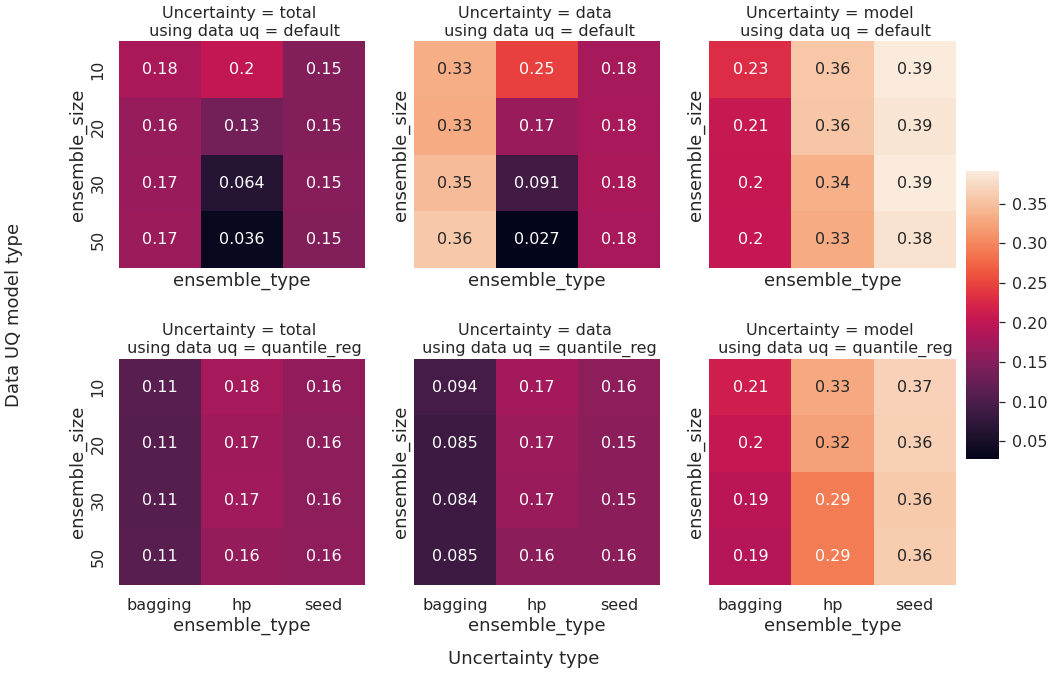
\includegraphics[width=0.95\linewidth]{figures/eval/uqlearn/regression-catboost-heatmap.png}
    \caption{Miscalibration area for different uncertainty types and data UQ models.}
    \label{fig:regression-catboost-heatmap}
\end{figure}

In figure \ref{fig:regression-catboost-results}, we observe that in terms of mean prediction performance, all CatBoost models are comparable with $0.89 \leq R2 \leq 0.93$. However, regarding UQ performance, disparities are present across models, and the hyper-parameter ensembles of size 50 appear to outmatch all other models. A larger ensemble size also has a positive impact on UQ performance for all metrics. Furthermore, model uncertainty systematically underperforms compared to total or data uncertainty. This can be further examined in figure \ref{fig:regression-catboost-heatmap} that highlights miscalibration scores for all different models in a heat map. The latter plot also allows us to investigate the performance divergence between intrinsic and extrinsic uncertainty models. In particular, quantile regression coupled with bagging or seed ensemble produces superior UQ models than their intrinsic counterparts. However, the intrinsic hyperparameter 50-ensemble eventually constitutes the best model with a miscalibration area of 0.027.

\begin{figure}[!htbp]
    \centering
    \begin{subfigure}[b]{0.99\textwidth}
         \centering
         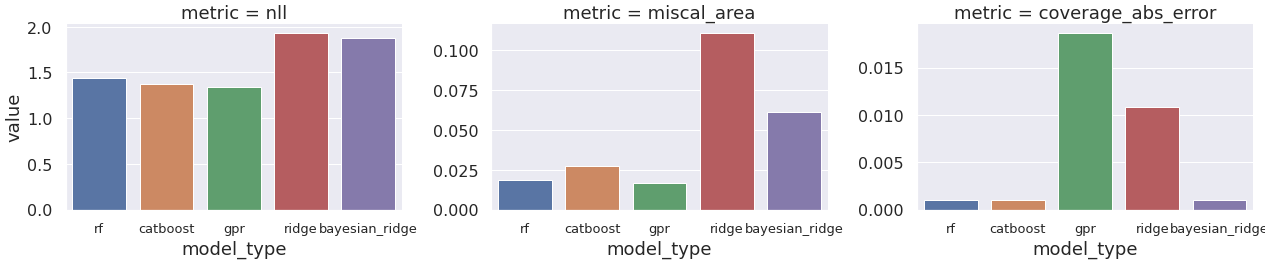
\includegraphics[width=\textwidth]{figures/eval/uqlearn/regression-best-models.png}
         \caption{Metrics scores for the best models.}
         \label{fig:regression-best-models-metrics}
     \end{subfigure}
     \hfill
     \begin{subfigure}[b]{0.99\textwidth}
         \centering
         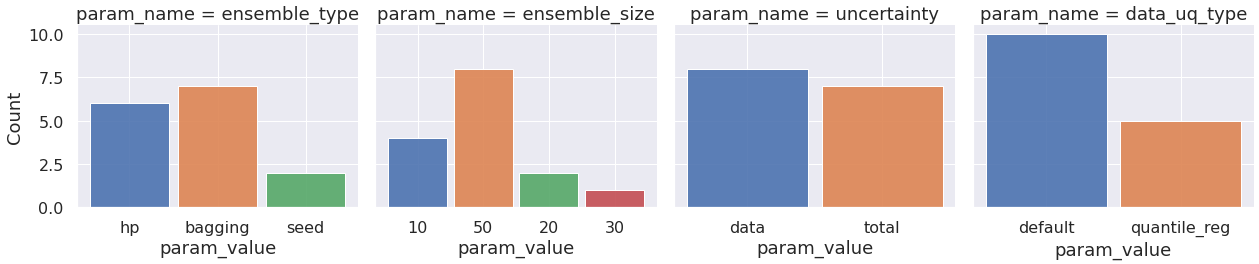
\includegraphics[width=\linewidth]{figures/eval/uqlearn/regression_param_hist.png}
         \caption{Distribution of the best hyperparameters. }
         \label{fig:regression-hyperparam-hist}
     \end{subfigure}
     \caption{Summary plots for the best regression estimators.}
     \label{fig:regression-best-models}
\end{figure}


An equivalent analysis can be conducted for all different base model types. A summary of the best UQ models for each metric is displayed in figure \ref{fig:regression-best-models-metrics}. Random Forest, GBT and Gaussian Process are similar in terms of performance and outperform both Ridge and Bayesian Ridge regression models. In figure \ref{fig:regression-hyperparam-hist}, the distribution of the hyperparameters leading to these best models is plotted. Overall, intrinsic data UQ, coupled with large size (e.g. 50) hyper-parameter or bagging UQ ensembles, give rise to decent UQ models for the Boston Housing dataset. 


\subsection{Classification}


A similar analysis is conducted for classification models. However, no distinction is made between total, data and model uncertainty because most evaluation metrics are solely based on class probabilities. In contrast with entropy, the latter cannot be decomposed into different uncertainty parts. This allows us to study the performance of different models in a single plot as shared in figure \ref{fig:classification-results}. As it was already the case on the regression dataset, in terms of F1 score, all models are comparable. However, the uncertainty quantification metrics inform us that ensemble size has a weaker impact on performance compared to the regression case. Furthermore, GBT usually leads to the best UQ models, as shown in figure \ref{fig:classification-best-models}.



% no difference between data and model uncertainty because the metrics used only consider probabilities and not entropies 

\begin{figure}[!htbp]
    \centering
    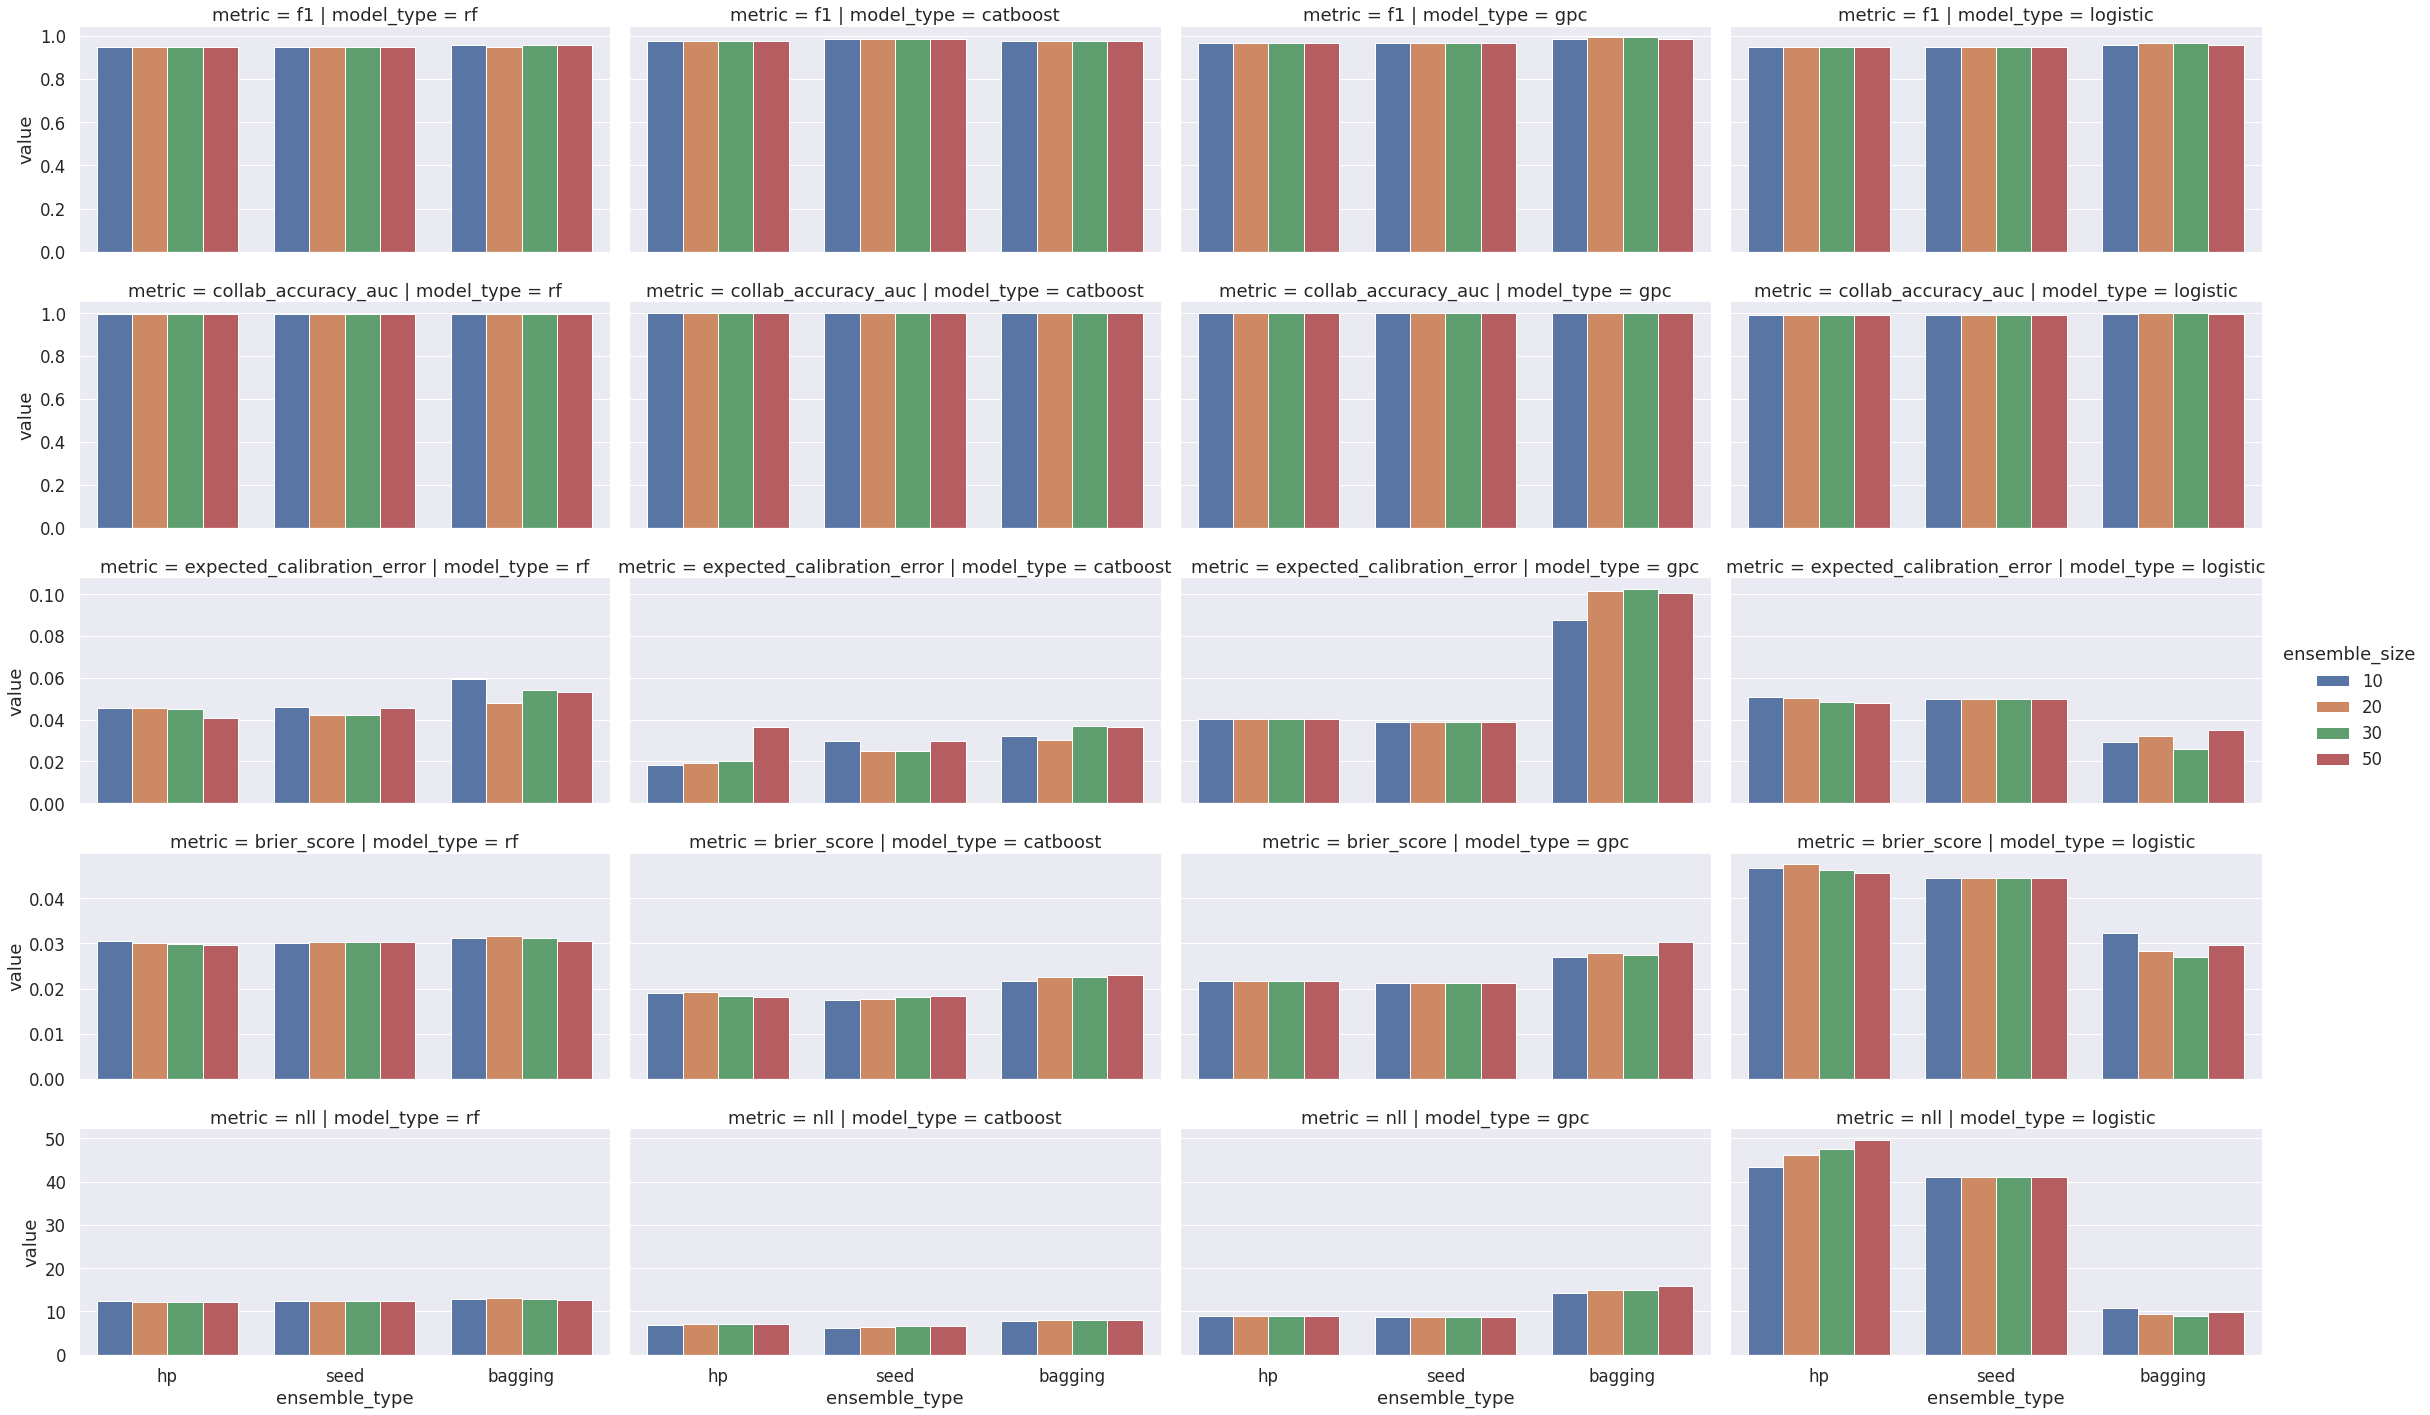
\includegraphics[width=1.1\linewidth]{figures/eval/uqlearn/classification-results.png}
    \caption{Results of classification experiment.}
    \label{fig:classification-results}
\end{figure}

\begin{figure}[!htbp]
    \centering
    \begin{subfigure}[b]{0.99\textwidth}
         \centering
         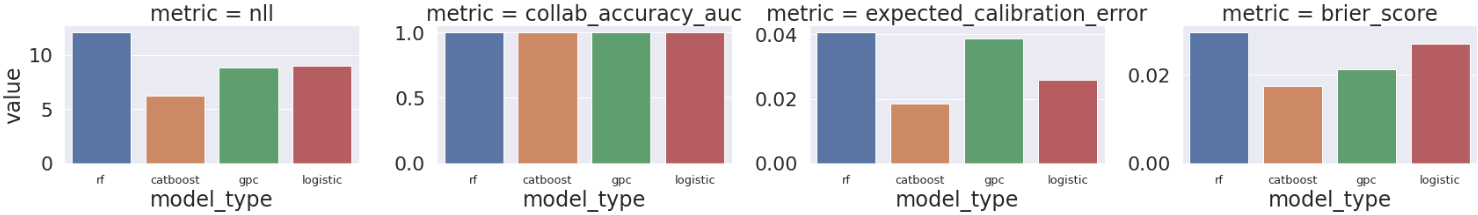
\includegraphics[width=\textwidth]{figures/eval/uqlearn/classification-best-models.png}
         \caption{Metrics scores for the best models.}
         \label{fig:classification-best-models-metrics}
     \end{subfigure}
     \hfill
     \begin{subfigure}[b]{0.99\textwidth}
         \centering
         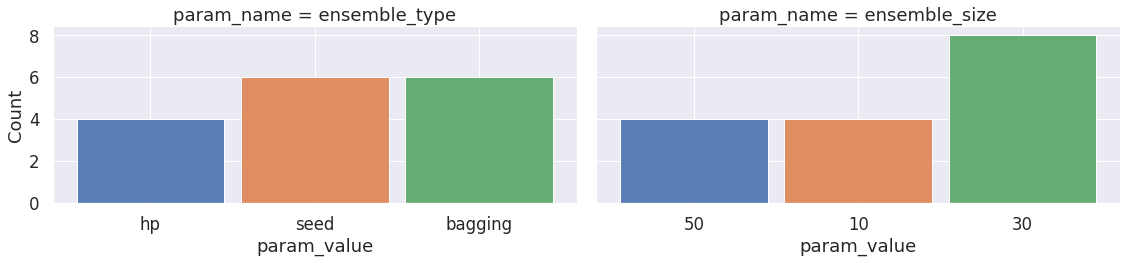
\includegraphics[width=\linewidth]{figures/eval/uqlearn/classification-param-hist.png}
         \caption{Distribution of the best hyperparameters. }
         \label{fig:classification-hyperparam-hist}
     \end{subfigure}
     \caption{Summary plots for the best classification estimators.}
         \label{fig:classification-best-models}
\end{figure}


%TODO
%\subsection{Clustering}


\section{Out-of-distribution evaluation} \label{experiment:OOD-evaluation}

In the previous section, the evaluation of UQ models was focused on in-distribution data. Indeed, the test set was constructed from the same underlying distribution as the training data. However, in production environments, out-of-distribution (OOD) examples are frequent, and it is important to be able to rely on the output of UQ models in these scenarios, especially if the performance of the model drops.
%might drop significantly when evaluated on these special data points. 
\newpage
In the benchmark datasets described in section \ref{section:datasets}, no extra OOD test set is available to perform such an evaluation. Consequently, it is first required to generate these OOD data points. Different types of perturbations $\delta$ with intensity $\epsilon$ for a given dataset $D_{test} = (X,Y) =\{(x_i,y_i)\}_{i=1}^N$ are considered:

\begin{itemize}
    \item White noise perturbations: $\delta = \epsilon \cdot \Normal(0, Var(X))$
    \item Fast-Gradient-Sign Perturbations\cite{FGSM} (FGSM): $\delta = \epsilon \cdot Sign\left(\nabla_X \Loss(f(X), Y)\right)$
    \item Uncertainty-Driven Perturbations\cite{UDP} (UDP): $\delta = \epsilon \cdot Sign\left(\nabla_X \Entropy(f(X)) \right)$
\end{itemize}

The OOD test set is defined as $D_{OOD} = (X + \delta, Y)$. In figure \ref{fig:adversarial-evaluation}, the evolution of the accuracy, the calibration error and the mean entropy over the OOD test predictions are displayed as functions of the attack step size $\epsilon$ for a Logistic Regression model on the breast cancer dataset. The model seems to be relatively robust against white noise attacks. The fast-gradient-sign perturbations are more harmful since the accuracy drops below the $50\%$ threshold with a step size of $0.15$. However, although the model makes more mistakes, it is also more confident about its predictions. This indicates a failure of the model to evaluate its uncertainty on OOD data. Indeed, the $ECE$ increases significantly, and after a short growth phase (i.e. $\epsilon < 0.1)$, the mean entropy quickly reaches the minimum level.
% ensembling does provide a better performance 
% idea metric: the area below current max curve; if the curve is strictly increasing, it is 0.
\begin{figure}
    \centering
    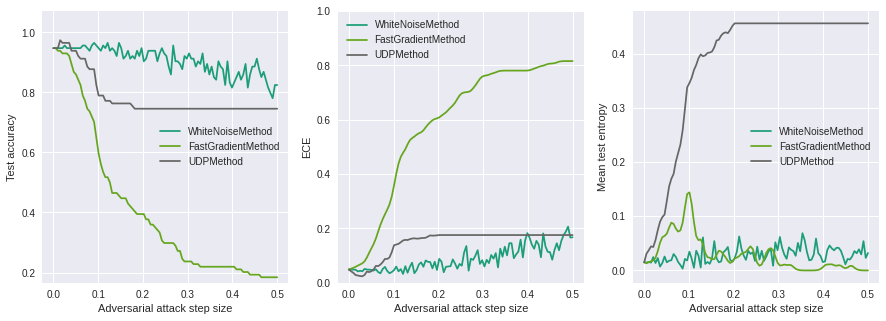
\includegraphics[width=\linewidth]{figures/eval/eval_adv_uq.png}
    \caption{Adversarial evaluation of a Logistic Regression model (breast cancer dataset).}
    %The robustness of the model is tested against three different attack types.
    \label{fig:adversarial-evaluation}
\end{figure}

\begin{figure}[!htbp]
    \begin{subfigure}{\textwidth}
      \centering
      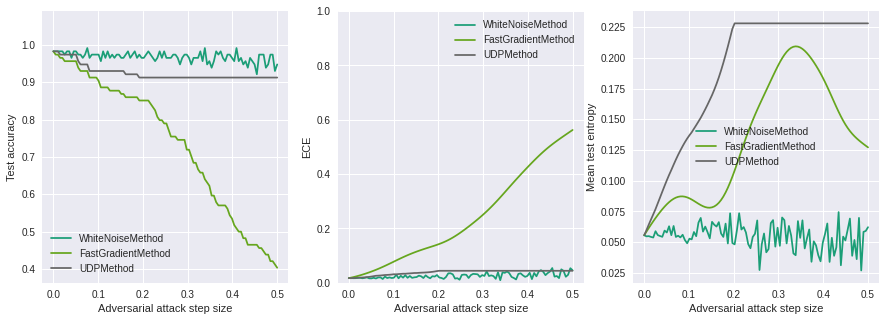
\includegraphics[width=\linewidth]{figures/eval/eval_adv_uq_train_noise.png}
      \caption{Adversarial training on the white noise attack.}
    \end{subfigure}
     \begin{subfigure}{\textwidth}
      \centering
      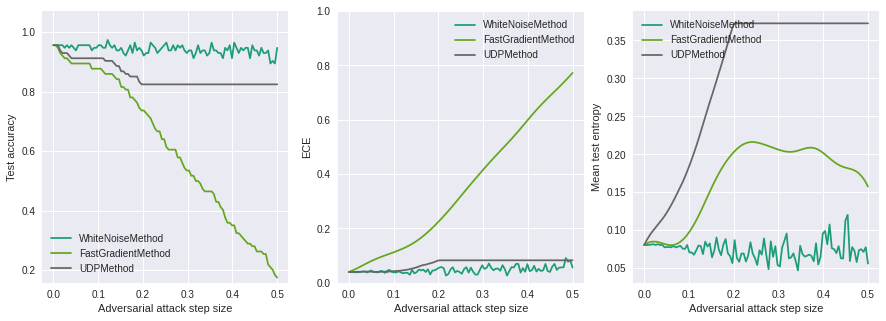
\includegraphics[width=\linewidth]{figures/eval/eval_adv_uq_train_fgsm.png}
      \caption{Adversarial training on the FGSM attack.}
    \end{subfigure}
     \begin{subfigure}{\textwidth}
      \centering
      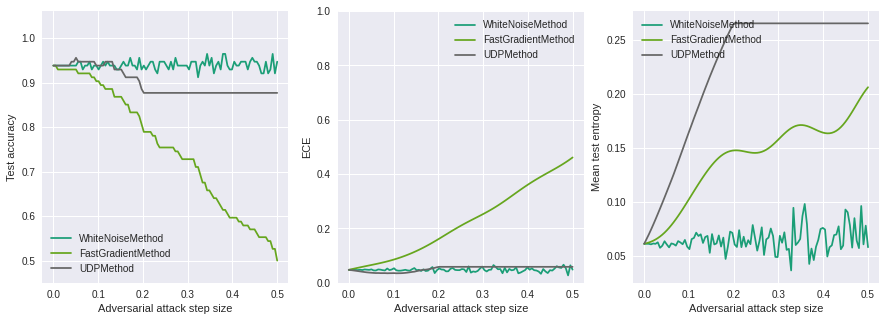
\includegraphics[width=\linewidth]{figures/eval/eval_adv_uq_train_udp.png}
      \caption{Adversarial training on the UDP attack.}
    \end{subfigure}
    \caption{Evaluation of an Adversarial Logistic Regression model (breast cancer dataset).}
    \label{fig:adversarial-evaluation-training}
\end{figure}

% adversarial ensembles 

\begin{figure}[!htbp]
    \begin{subfigure}{\textwidth}
      \centering
      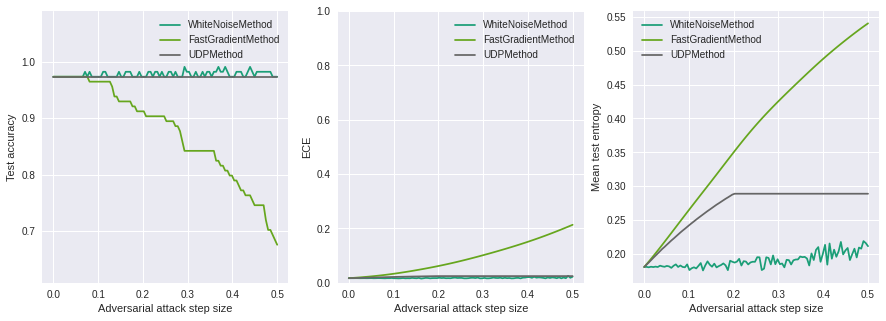
\includegraphics[width=\linewidth]{figures/eval/eval_adv_uq_train_ensemble_fgsm_mean.png}
     \caption{Evaluation on ensemble $mean$ attacks.}
    \end{subfigure}
    % \begin{subfigure}{\textwidth}
    %  \centering
    %  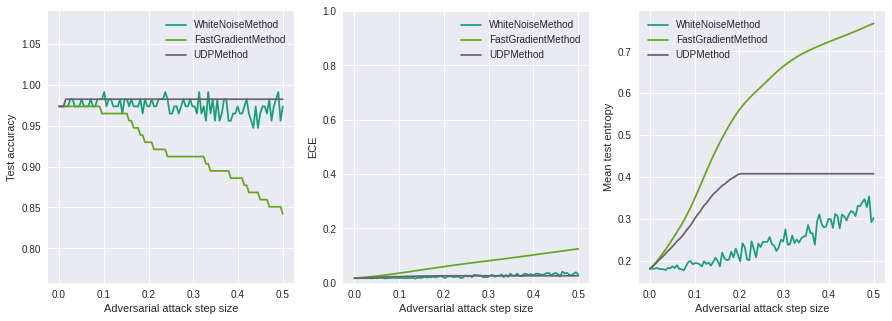
\includegraphics[width=\linewidth]{figures/eval/eval_adv_uq_train_ensemble_fgsm_first.png}
    %  \caption{Adversarial training on the ensemble first FGSM attack}
    %\end{subfigure}
     \begin{subfigure}{\textwidth}
      \centering
      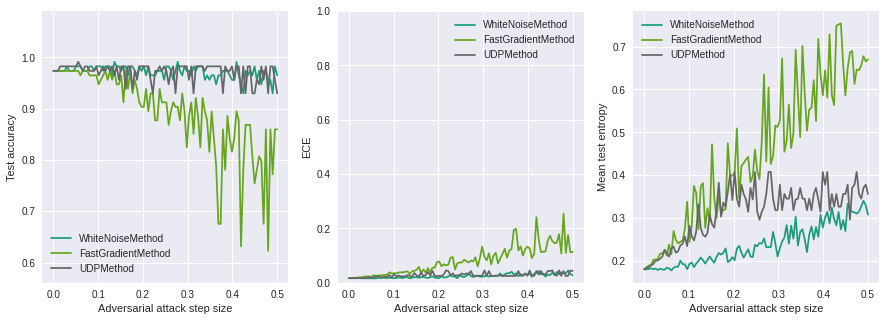
\includegraphics[width=\linewidth]{figures/eval/eval_adv_uq_train_ensemble_fgsm_random.png}
      \caption{Evaluation on ensemble $random$ attacks.}
    \end{subfigure}
    \begin{subfigure}{\textwidth}
      \centering
      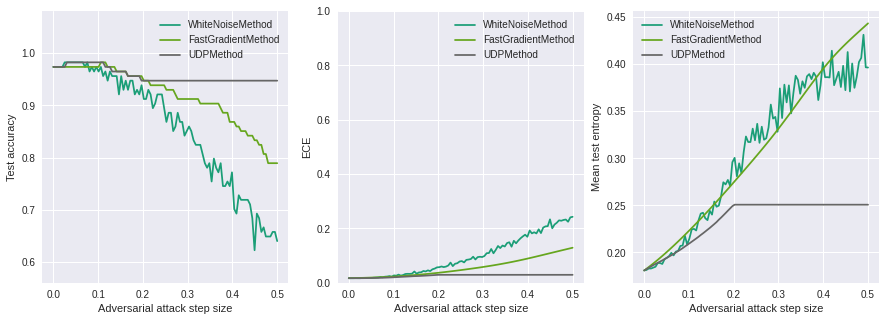
\includegraphics[width=\linewidth]{figures/eval/eval_adv_uq_train_ensemble_fgsm_max.png}
       \caption{Evaluation on ensemble $max$ attacks.}
    \end{subfigure}
    \caption{Evaluation of an Adversarial ensemble composed of 10 Logistic Regression models (breast cancer dataset). It is trained only on the FGSM attack.}
    \label{fig:adversarial-evaluation-training-ensemble-fgsm}
\end{figure}

This motivates the introduction of adversarial training (cf. algorithm \ref{alg:adversarial-training}) for uncertainty quantification to equip models with tools to handle OOD data points. The results of the adversarial training procedure of a Logistic Regression model are shown in figure \ref{fig:adversarial-evaluation-training}. Models are trained against one specific type of attack and evaluated on all attack types to assess generalisation. We observe that adversarial training on any attack improves the robustness of the model on all attacks: models are better calibrated and suffer less from overconfident incorrect predictions. In addition, robustness can be further improved by ensembling independently trained adversarial models. The latter models are evaluated on ensemble attacks aggregated using a $mean$, $random$ and $max$ aggregation function (cf. section \ref{section:design:adversarial} for more information about these attacks). Due to space constraints, only results on FGSM ensemble attacks are shared in this section. Still, the results can be generalised to other types of attacks, as shown in appendix \ref{appendix:adversarial-ensemble-plots}. From that experiment, we concluded that adversarial ensembles offer the strongest robustness against out-of-distribution data points. 


%- Evaluated 
%- Training an ensemble is also robust to different types of attacks (mean, first, %random, max).
%- Study how well training on a single perturbation influences the output.
%- Consider a single model: Logistic Regression. 


%\section{UQ in class imbalance settings}
% TODO


\section{Graph-to-text models}


\subsection{Evaluation of existing graph-to-text models} \label{experiment:G2T-raw-performance}
% exploration of hallucinations in both datasets
% report bleu scores of models
% observations: less hallucination of the predictions than reference text
\begin{table}[ht]
\centering
\caption{Performance of graph-to-text models on test set.}
\label{table:G2T-models}
\begin{tabular}[t]{lcclc} % p{3cm}
\toprule
Model & Bleu & Rouge & Faithfulness (fined-tuned NER) & Number faithfulness \\
\midrule
T5-base-WebNLG     & 0.632 & 0.744 & 0.996         & 0.972 \\
T5-small-WebNLG    & 0.626 & 0.740 & 0.995         & 0.966 \\
T5-base-SAR        & 0.511 & 0.588 & 0.763 (0.883) & 0.444 \\
T5-small-SAR       & 0.531 & 0.606 & 0.764 (0.876) & 0.473 \\
\bottomrule
\end{tabular}
\end{table}%

 The evaluation presented in this section is based on several T5 graph-to-text models trained on the WebNLG and SAR datasets. The performance of these models can be found in table \ref{table:G2T-models}. For the SAR dataset, faithfulness is evaluated using two different NER models: first, the base \textit{spaCy} model and, secondly, a fined-tuned model previously trained by a colleague at Oracle. More details about this NER model are available in appendix \ref{appendix:custom-ner-sar}.



In addition, table \ref{table:G2T-models-faithfulness} compares the hallucination ratio for model predictions and reference texts on the train and test sets. In contrast with the results of Dziri et al.\cite{originHalluDataOrModel}, the evaluation suggests that hallucinations are not amplified during testing compared to training. Furthermore, hallucinations appear slightly more frequently in the reference texts than in the actual model predictions. From a manual exploration of hallucinations occurring in the WebNLG and SAR datasets, a possible explanation could be human labelling errors in the reference texts that are not reproduced in the predictions. Some of them are highlighted in table \ref{table:G2T-models-errors}. Finally, the rather important number of hallucinations present in the SAR dataset (both reference texts and predictions) can be traced back to an issue in the data-gathering process. Indeed, several pieces of information available in the reference text cannot be found in the input graph (e.g. age of the persons of interest in the report). Hence, it is never possible for the model to produce a factual prediction for such elements. Additional edge types need to be included in the graph to mitigate this problem.

\begin{table}[!ht]
\centering
\caption{Comparison of hallucination ratios in graph-to-text models.}
\label{table:G2T-models-faithfulness}
\begin{tabular}[t]{lllcc} % p{3cm}
\toprule
 &  \multicolumn{2}{c}{$r_h$ (fined tuned NER)} & \multicolumn{2}{c}{$r_h^{num}$} \\
 \cmidrule(rl){2-3} \cmidrule(rl){4-5}
   Model  & train & test & train & test  \\
\midrule
Reference-WebNLG   & 0.016 & 0.011 & 0.039 & 0.040\\ 
T5-base-WebNLG     & 0.004 & 0.004 & 0.029 & 0.028\\
T5-small-WebNLG    & 0.007 & 0.005 & 0.034 & 0.034\\
Reference-SAR      & 0.254 (0.112) & 0.237 (0.107) & 0.561 & 0.582 \\ 
T5-base-SAR        & 0.254 (0.112) & 0.237 (0.117) & 0.564 & 0.556  \\
T5-small-SAR       & 0.253 (0.112) & 0.236 (0.124) & 0.562 & 0.527 \\
\bottomrule
\end{tabular}
\end{table}%


\begin{table}[!ht]
\centering
\caption{Examples of human labelling errors in WebNLG dataset.}
\label{table:G2T-models-errors}
\begin{tabular}[t]{cp{5cm}p{5cm}} % 
\toprule
Id & Graph edge & Reference text   \\
\midrule
0 & <H> 1097 Vicia <R> epoch is <T> \textbf{2006-12-31} & The epoch of 1097 Vicia is on \textbf{13 January 2016}. \\ 
1 & <H> Abradab <R> associated band/associated musical artist is <T> \textbf{Magik} (rapper) & He is with rapper associated with \textbf{Magri}. \\
\bottomrule
\end{tabular}
\end{table}%

\subsection{Relationship between entropy and hallucinations} \label{experiment:relation-entropy-hallucination}

This experiment aims to demonstrate whether or not a relationship between uncertainty and hallucination occurrence exists. Different UQ models lead to different uncertainty scores, impacting, in turn, hallucination detection performance. We provide insights into how the results are affected by the choice of UQ models. This experiment will also validate the introduction of the $MHE$ and $MHED$ metrics to evaluate UQ models.

To study the relationship between entropy and hallucination, the model $f$ is evaluated on both $D = \{(G_i, T_i)\}_i$ and the corresponding hallucination dataset $\Tilde{D} = \{(\Tilde{G_i}, T_i, a_i\}_i$. Given an input graph, i.e. $G_i$ or $\Tilde{G_i}$, the prediction entropy sequence is computed when the model is forced to re-generate the reference text $T_i$. Indeed, hallucination labels $a^i$ are paired up with the reference texts $T_i$ and are therefore useless if a brand new prediction $\hat T_i = f(G_i)$ is created. To force the model to re-generate $T_i$, the targeted decoding procedure defined in algorithm \ref{alg:targeted-decoding} is used. Let $\Entropy_i^D = \{ \Entropy_{i,j}^D \}_j = \{ \Entropy_{j}(G_i, T_i) \}_j$ be the entropy sequences generated using targeted decoding on dataset $D$. Let $\delta^D$ be the mean hallucination entropy difference (MHED) on dataset $D$ :

\begin{equation}
    MHED_i = \delta_i^D = \frac{\sum_j a_{i,j} \cdot \Entropy_{i,j}^D}{\sum_j a_{i,j}} - \frac{\sum_j \neg a_{i,j} \Entropy_{i,j}^D}{\sum_j \neg a_{i,j}}
\end{equation}


It allows us to compute the accepted hallucination noise level $\epsilon = \mu(\delta^D) = \frac{1}{N} \sum_n \delta^D_i $ since $D$ is not a hallucination dataset. This can be extended to the hallucination dataset $\Tilde{D}$ using the notation $\delta^{\Tilde{D}}_i$. The condition $s_i = I\{\delta^{\Tilde{D}}_i > \epsilon\}$ provides evidence that the model produced a higher entropy for hallucination tokens given the input graph $\Tilde{G_i}$. The robust condition $v_i =  I\left\{\delta^{\Tilde{D}}_i > \epsilon_{0.95}\right\}$ at 95\% confidence is also computed so that $\epsilon_{0.95} = \epsilon + 1.96 \frac{\sigma(\delta^D)}{\sqrt{N}}$.
% results
The results of this experiment are shared in table \ref{table:relationship-entropy-uncertainty}. The evaluation is performed on a truncated version of the test set where data points containing no hallucination have been dropped, e.g. $\{i \;:\; \forall_j \;a_{i,j} = 0\}$. We observe that the hallucination entropy difference on the hallucination dataset is significantly higher than on the non-hallucination one. This supports the claim that entropy is high for hallucination tokens compared to non-hallucinated ones. For the WebNLG dataset, $\mu(v) = 0.936$, i.e. for 93.6\% of the data points the claim holds. For the SAR dataset, the ratio is increased to 100\%. 


\begin{table}[ht]
\centering
\caption{Mean hallucination entropy difference for different test datasets. }
\label{table:relationship-entropy-uncertainty}
\begin{tabular}[t]{lcccccccc} % p{3cm}
\toprule
 & & \multicolumn{3}{c}{Dataset $D$} & \multicolumn{4}{c}{Hallucination dataset $\Tilde{D}$} \\
 \cmidrule(rl){3-5} \cmidrule(rl){6-9}
Model      &  $N$   & $\mu(\delta^D)$ & $\sigma(\delta^D)$ & $\epsilon_{0.95}$ & $\mu(\delta^{\Tilde{D}})$ & $\sigma(\delta^{\Tilde{D}})$ & $\mu(s)$ & $\mu(v)$  \\
\midrule
T5-base-WebNLG     & 530 & -0.30 & 0.50 & -0.23 & 1.16 & 0.95 & 0.943 & 0.936 \\
T5-base-SAR         & 21 & -0.02 & 0.07 & 0.01 & 0.20 & 0.11 & 1.000 & 1.000 \\
\bottomrule
\end{tabular}
\end{table}%

\subsection{Factual uncertainty evaluation of graph-to-text models}

In section \ref{experiment:relation-entropy-hallucination}, a relationship between uncertainty and hallucinations was established. It motivated the use of the factual uncertainty metrics introduced in section \ref{experiment:relation-entropy-hallucination} to evaluate the quality of UQ in a graph-to-text use case. Table \ref{table:UQ-G2T-models} contains the results of this evaluation for the mean hallucination entropy ($MHE$) and mean hallucination entropy difference ($MHED$) metrics. In addition, $MHED*$, a modified version of $MHED$, where all stop words and punctuation tokens have been dropped, is also reported.  

Predictions are generated using the targeted decoding (cf. algorithm \ref{alg:targeted-decoding}) to reproduce the reference texts of the test set. On both WebNLG and SAR datasets, the dropout ensemble outmatches the remaining ensemble models independently of the uncertainty type. Surprisingly, graph-encoding ensemble performs worse than a UQ model without an ensemble. This indicates that randomly shuffling the ordering of edges could negatively impact the performance of the graph-to-text generation process.
% report metrics of UQ models: calibration
% discuss MHED* metric
% targeted decoding to generate output

\begin{table}[!ht]
    \centering
        \caption{Factual performance of UQ graph-to-text models on test set.}
    \label{table:UQ-G2T-models}
     \centerline{
    \begin{tabular}{clccccccccc}
\toprule
& & \multicolumn{3}{c}{$MHE$} & \multicolumn{3}{c}{$MHED$} & \multicolumn{3}{c}{$MHED*$} \\
    \cmidrule(rl){3-5} \cmidrule(rl){6-8} \cmidrule(rl){9-11}
&Uncertainty &         data & model & total &         data & model & total &                           data & model & total \\
&Ensemble          &              &       &       &              &       &       &                                &       &       \\
\midrule
\multirow{3}{*}{\rotatebox{90}{WebNLG}}
& None           &  ---  &  ---  &	2.07 & 	--- & --- & 1.30  & --- 	&--- & 1.47 \\
& Graph encoding       &  1.82 &  0.01 &  1.84 &  1.28 &  0.01 &  1.29  &                       1.42 &  0.01 &  1.43  \\
& Deep           &  2.02 &  0.12 &  2.14 &  1.29 &  0.08 &  1.37  &                       1.45 &  0.09 &  1.54  \\
& Dropout        &  \textbf{2.15} &  \textbf{0.30} &  \textbf{2.45} &  \textbf{1.46} &  \textbf{0.23} &   \textbf{1.69} &                       \textbf{1.60} &  \textbf{0.24} &   \textbf{1.84} \\
% Dropout        &   \textbf{2.17 (0.1)} &  \textbf{0.30} &  \textbf{2.47} &  \textbf{1.46 (0.16)} &  0.22 &  \textbf{1.68} &                    \textbf{1.59 (0.12)} &  0.23 &  \textbf{1.82} \\
%&Encoding &  1.87 (-0.2) &  0.01 &  1.89 &  1.31 (0.01) &  0.01 &  1.32 &                   1.44 (-0.03) &  0.01 &  1.45 \\
%&Seed           &  2.13 (0.06) &  0.31 &  2.43 &  1.45 (0.15) &  \textbf{0.23} &  \textbf{1.68} &                    1.58 (0.11) &  \textbf{0.24} &  \textbf{1.82 }\\
\\
\multirow{3}{*}{\rotatebox{90}{SAR}}
& None           & ---	 &  ---  & 	0.86  & ---  & --- &	0.72 &	--- & --- & 0.70 \\
& Graph encoding       &  0.71 &  0.09 &   0.80 &  0.63 &  0.08 &  0.71  &                       0.63 &  0.08 &  0.70 \\
& Deep           &  0.74 &  0.41 &  1.15  &  0.62 &  0.35 &   0.97  &                       0.60 &  0.34 &  0.95 \\
& Dropout        &  \textbf{0.97} &  \textbf{0.49} &   \textbf{1.46} &  \textbf{0.83} &  \textbf{0.41} &   \textbf{1.24} &                       \textbf{0.82} &  \textbf{0.41} & \textbf{ 1.22} \\




%Dropout        &    0.4 (0.06) &  0.20 &  0.60 &   0.26 (0.05) &  0.12 &  0.38 &                0.25 (0.06) &  0.12 &  0.37 \\
%&Encoding &  0.25 (-0.09) &  0.03 &  0.28 &  0.17 (-0.04) &  0.02 &  0.19 &               0.17 (-0.02) &  0.02 &  0.18 \\
%&Seed           &    0.4 (0.06) &  0.20 &  0.59 &   0.26 (0.05) &  0.12 &  0.38 &                0.25 (0.06) &  0.12 &  0.37 \\


\bottomrule
\end{tabular}
}
\end{table}


\subsection{Entropy predictive power} \label{experiment:entropy-predictive-power}

The experiment of section \ref{experiment:relation-entropy-hallucination} has established the validity of the synthetic datasets as well as the relationship between uncertainty and hallucination occurrence. In this section, we formally evaluate the predictive power of entropy when it comes to token hallucination detection using the models defined in section \ref{design:hallucination-detection-models}:
\begin{itemize}
    \item Baseline hallucination detection based on NER. No model training or synthetic hallucination dataset is required with this approach.
    \item Logistic regression models based on different sets of features:
    \begin{itemize}
        \item Total uncertainty of the current token.
        \item Model and data uncertainty of the current token.
        \item Total uncertainty of the past five tokens (sequence model).
        \item Model and data uncertainty of the past five tokens (split uncertainty sequence model).
    \end{itemize}
\end{itemize}
The uncertainty of the model is compared across different model types: base, graph encoding, dropout, and a deep-seed ensemble, all of size 5. Word expansion (cf. section \ref{design:synthetic-hallucination-data}) is also applied to the best of these models as a post-processing step.

\begin{figure}[!ht]
    \centering
    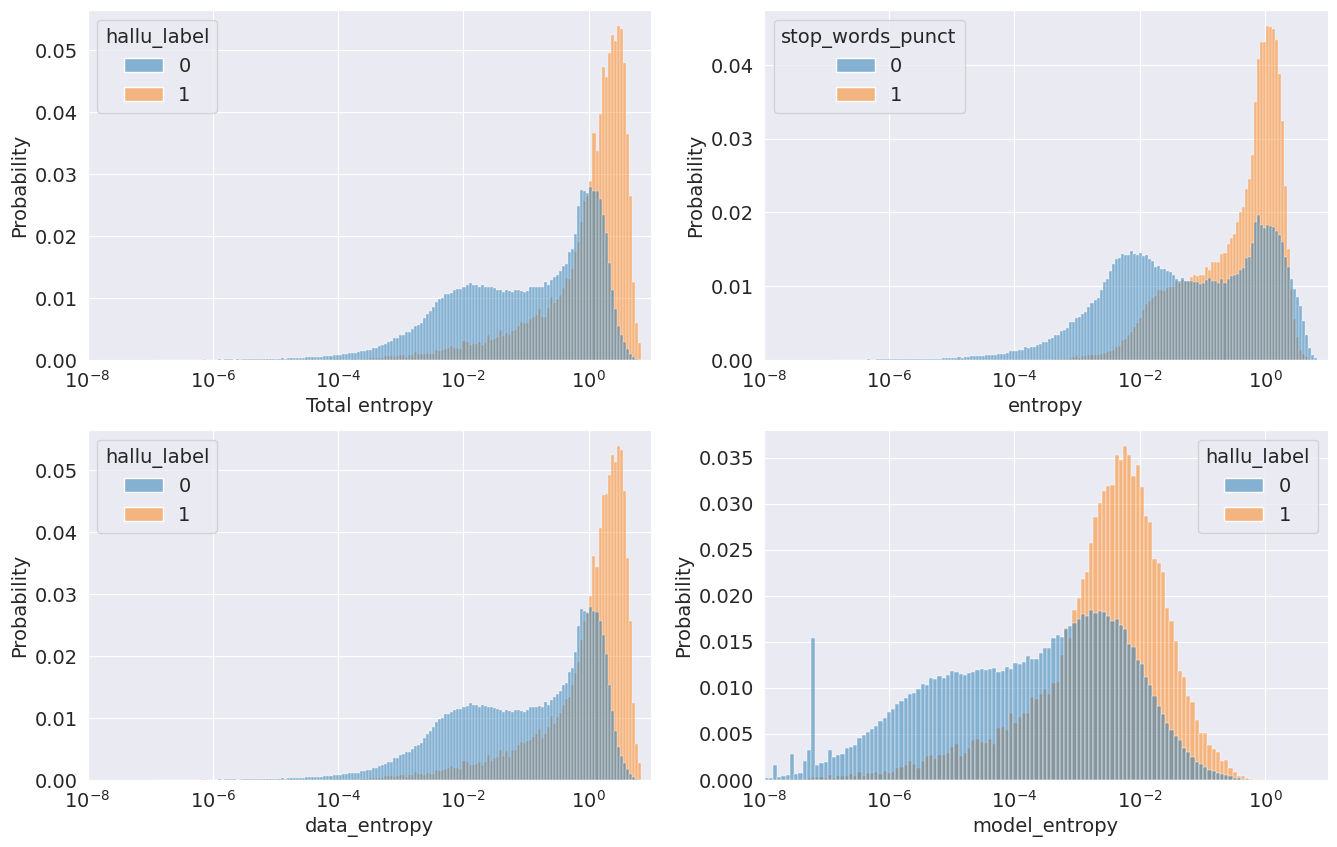
\includegraphics[width=0.85\linewidth]{figures/eval/entropy_pred_power/entropy_hist.png}
    \caption{Various histograms of token-level entropy (data, model and total) on the WebNLG dataset based computed using graph encoding ensembles.}
    \label{fig:entropy-hists}
\end{figure}

First, a simple data exploration step is carried out to visualise the entropy distribution for hallucination and non-hallucination tokens (cf. figure \ref{fig:entropy-hists}) based on the graph ensemble entropy predictions. The distributions of total entropy and data entropy are relatively similar, and a substantial probability mass can be witnessed for hallucination tokens with high entropies. This is less apparent for model entropy which could result in a smaller predictive power for this particular feature. In the top-right plot, the entropy distribution is also displayed for stop-words and punctuation tokens compared to other tokens. Intrinsically, stop-words and punctuation tokens do not meet the requirements to be considered hallucination or knowledge expression. However, the figure indicates significantly high entropies for these tokens. We decided to filter them out to improve the quality of the binary classification model. Given the spread of the x-axis in these plots, log and standard scaling preprocessing steps are applied to the entropy features. Similar conclusions can be drawn for the SAR dataset. 
% more on imbalance datasets



Besides, this classification task is strongly imbalanced, i.e. only 5.3\% of tokens are hallucination tokens for the WebNLG dataset and 1.6\% for the SAR dataset. The non-hallucination labels are also noisy. Indeed, some hallucinations are already present in the raw dataset, and they are not captured by the synthetic hallucination labels. Hence, false positives, e.g.  tokens that are not hallucinations but are predicted as such, are less critical than false negatives. Hence, recall is a more appropriate metric to consider than precision. When a strong imbalance is present, user-defined probability thresholds $T$, i.e. $\hat y_i = I\{p_{i,1} \geq T\}$, are commonly used to control better the number of acceptable false positives for each domain of applications.
For this reason, hallucination detection models are compared using Receiver Operating Characteristic (ROC) and Precision-Recall (PR) curves, for both datasets. Using the probabilistic interpretation of the $AUC-ROC$ metric, it can be shown that it is likely to be high for an imbalanced dataset. In contrast, $AUC-PC$ is better suited for such use cases and is the metric used to select the final model. 

\begin{figure}
     \centering
     \begin{subfigure}[b]{0.95\textwidth}
         \centering
         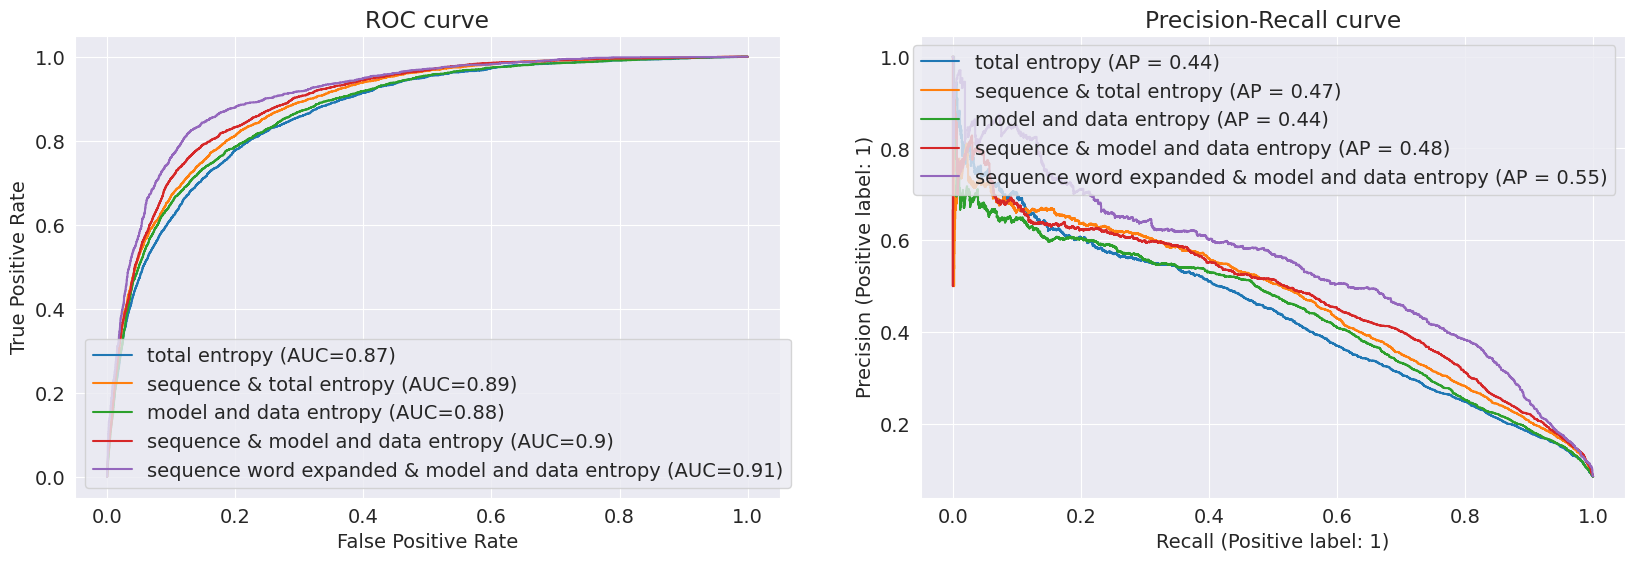
\includegraphics[width=\textwidth]{figures/eval/entropy_pred_power/WebNLG_dropout_ensemble.png}
         \caption{WebNLG dataset.}
         \label{fig:webnlg-local-ensemble-hallu-detection}
     \end{subfigure}
     \hfill
    \begin{subfigure}[b]{0.95\textwidth}
         \centering
         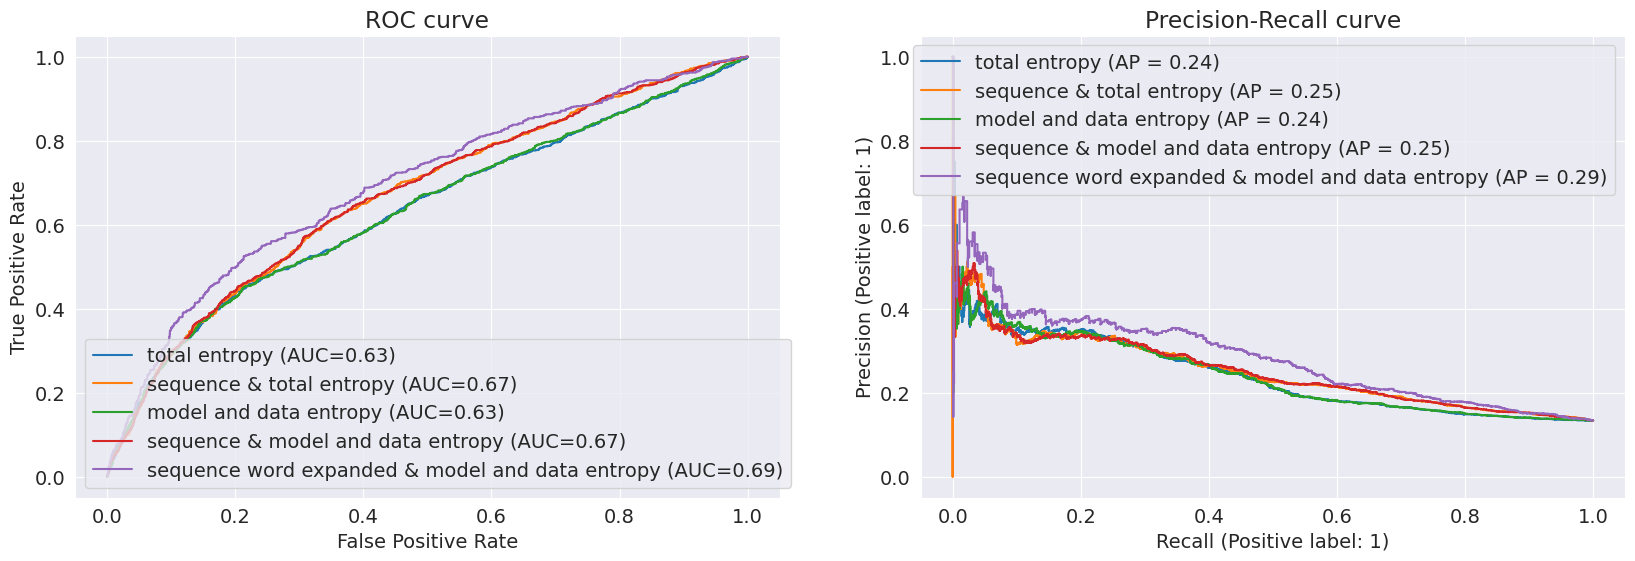
\includegraphics[width=\textwidth]{figures/eval/entropy_pred_power/SAR_hallu_dropout_results.png}
         \caption{SAR dataset.}
         \label{fig:sar-local-ensemble-hallu-detection}
     \end{subfigure}
     \hfill
     \hfill
       \caption{Comparison of Logistic regression models trained on various sets of features via $ROC$ and $PR$ curves. Entropies are generated using dropout ensemble}
        \label{fig:local-ensemble-hallu-detection}
\end{figure}
% table \ref{baseline-ner-hallucination-detection} contains 


In figure \ref{fig:local-ensemble-hallu-detection}, we observe that models achieving the best performance are those with the most extensive set of features, i.e. split uncertainty sequence models. The decomposition of total uncertainty into data and model components also leads to a slight improvement gap of around 0.01 in $AUC-PR$ for WebNLG but not SAR. Additionally, word expansion is a rather powerful tool as it increases the $AUC-PR$ score by 15\%. 

\begin{figure}[!ht]
     \centering
     \begin{subfigure}[b]{0.95\textwidth}
         \centering
         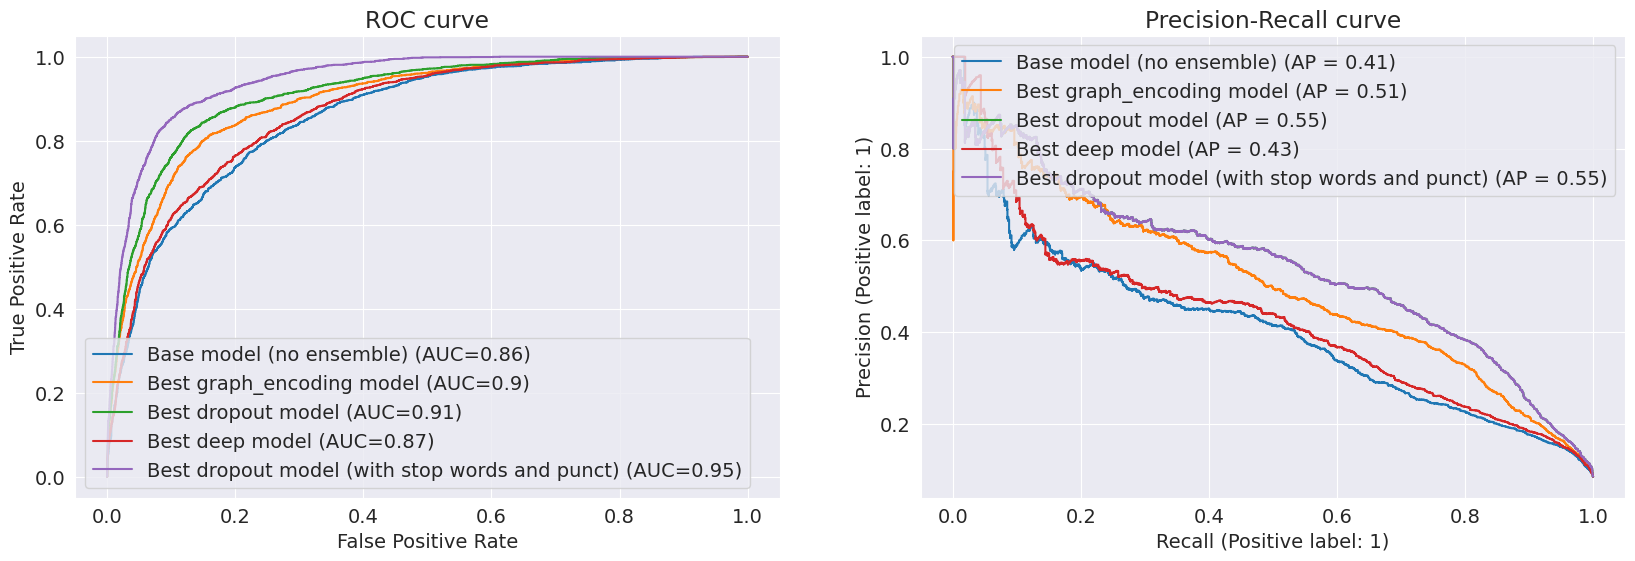
\includegraphics[width=\textwidth]{figures/eval/entropy_pred_power/webnlg_hd_results.png}
         \caption{WebNLG dataset.}
         \label{fig:webnlg-hallu-detection-best-results}
     \end{subfigure}
     \hfill
     \begin{subfigure}[b]{0.95\textwidth}
         \centering
         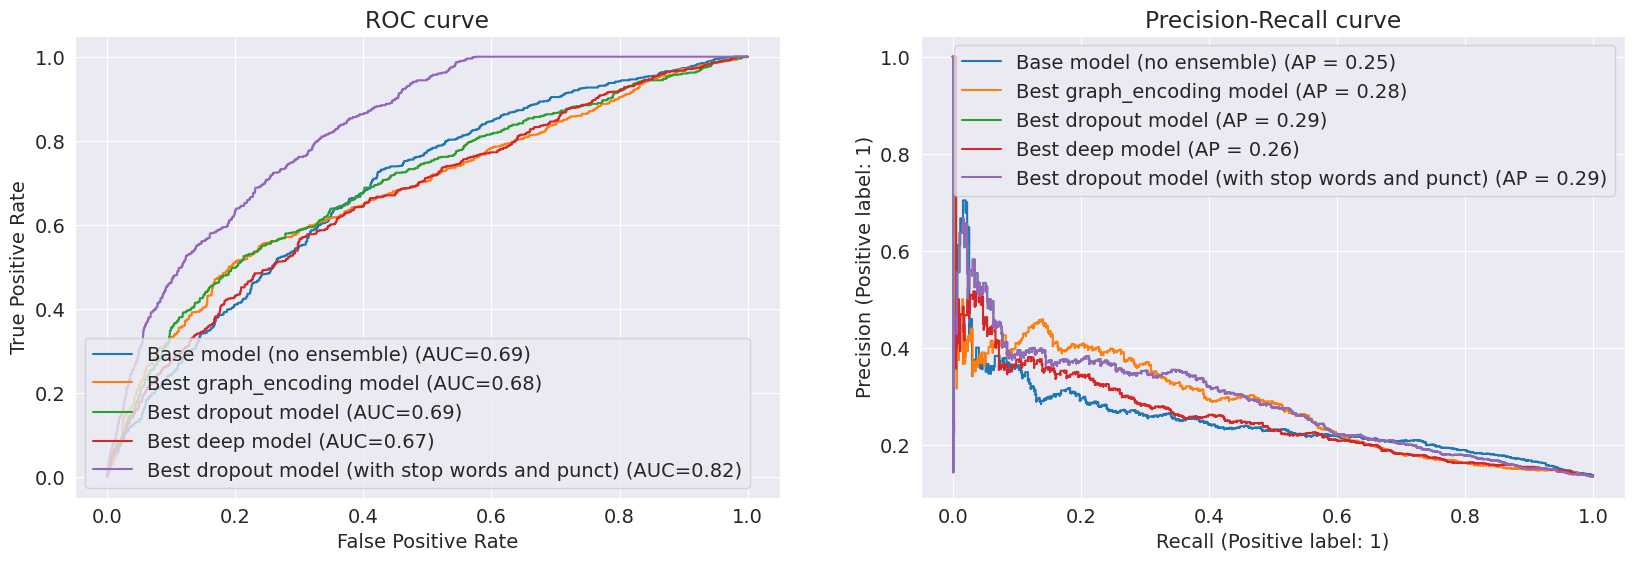
\includegraphics[width=\textwidth]{figures/eval/entropy_pred_power/SAR_hallu_results.png}
         \caption{SAR dataset.}
         \label{fig:sar-hallu-detection-best-results}
     \end{subfigure}
     \hfill
       \caption{Results of the entropy predictive power experiment. Split uncertainty sequence models generated by different ensemble UQ methods are compared.}
        \label{fig:experiment-hallu-detection}
\end{figure}

Figure \ref{fig:experiment-hallu-detection} extends this comparison to different ensembling techniques. Dropout ensembles obtain the best scores for both datasets. Surprisingly, deep seed ensembles do not reach their expected level of performance\cite{evalUQDatasetShift}. It would have been interesting to train these deep ensembles using more variations in the hyper-parameters and training schemes in the hope of bringing more variability in the output. However, given the time required to train and evaluate such models, as well as the time frame of this thesis, this is left as a future work step. Due to hallucinations present in the raw datasets, the precision of these models is not exceptionally high, as anticipated, especially for the SAR dataset. This can be explained by the larger hallucination ratio for the latter dataset (cf. \ref{table:G2T-models-faithfulness}).

Finally, table \ref{table:baseline-ner-hallucination-detection} summarises the performance of the best dropout ensemble models compared to baseline detection models based on named entity recognition. Entropy-based models generate better predictions than the baseline, which motivates further research to improve their quality.

\begin{table}[ht]
\centering
\caption{Comparison of NER and Ensemble-based hallucination detection models. Logistic regression predictions are generated using a threshold of $0.75$ for WebNLG and $0.40$ for SAR.}
\label{table:baseline-ner-hallucination-detection}
\begin{tabular}[t]{lcccccc} % p{3cm}
\toprule
& \multicolumn{3}{c}{Non-hallucination (label 0)} & \multicolumn{3}{c}{Hallucination (label 1)} \\
 \cmidrule(rl){2-4} \cmidrule(rl){5-7}
Model & precision & recall & f1-score & precision & recall & f1-score \\
\midrule
NER-baseline-WebNLG     &     0.93      & 0.91      & 0.92 &     0.17      & 0.21 & 0.19 \\
Dropout-ensembe-WebNLG & 0.99      &0.93   &   \textbf{0.96}  &     0.36    &  0.76   &   \textbf{0.48}  \\
NER-baseline-SAR        &      0.98    &  0.92   &  \textbf{ 0.95}   &  0.05      &0.21 &     0.08 \\
%0.87      & 0.91      & 0.89 &     0.21      & 0.16 & 0.18 \\
custom-NER-baseline-SAR &     1.00  &    0.83   &   0.91  &  0.10  &    0.94  &    0.18\\

Dropout-ensemble-SAR  & 0.95  &    0.93  &    0.94 &         0.34  &    0.39  &    \textbf{0.37} \\

%&  0.99  &    0.93  &    0.96   &     0.39  &    0.79 &     0.52\\

\bottomrule
\end{tabular}
\end{table}%



Examples of the binary predictions of the hallucination detection models are shown below for the WebNLG dataset. Hallucination ground truth labels are \textit{"Denmark"} and \textit{"Universitas Aarhusiensis"}. Using a rather conservative threshold of $0.75$, the following prediction is constructed:


\epigraph{
The School of Business and Social Sciences at the Aarhus University is located in Aarhus, Denmark, and it was established in 1928. Its dean is Thomas Pallesen, and it has 16,000 students. Its Latin name is "\textcolor{BrickRed}{\textbf{Universitas Aarhusiensis}}". It is affiliated to the European University Association.
}{Dropout ensemble prediction with probability threshold $0.75$}

At token-level, the precision is 1.00, and the recall is 0.9. However, even if the graph does not contain an edge about Denmark, one might argue that the language model could infer that information from the city of Aarhus. By setting a lower value threshold, e.g. 0.5, recall improves to $1.00$ to the detriment of precision which goes down to $0.59$:

\epigraph{
The School of Business and Social Sciences at the Aarhus University is located in \textcolor{BrickRed}{\textbf{Aarhus, Denmark}}, and it was established in 1928. Its \textcolor{BrickRed}{\textbf{dean}} is Thomas Pallesen, and it has 16,000 students. Its \textcolor{BrickRed}{\textbf{Latin}} name is "\textcolor{BrickRed}{\textbf{Universitas Aarhusiensis}}". It is \textcolor{BrickRed}{\textbf{affiliated}} to the European University Association.
}{Dropout ensemble prediction with probability threshold $0.50$} 
